\section{Appendix}

\subsection{Notation}

\begin{tabular}{ll}   
  \toprule
  Symbol & Meaning\\
  \midrule
  $\state \in \State$ & State $\state$ in state space $\State$ \\
  $\act \in \Action$ & Action $\act$ in Action space $\Action$ \\
  $\rew \in \R$ & Observed reward \\
  $\goal \in \Goal$ & Goal $\goal$ in goal space $\Goal$ \\
  $f_\goal(\state_t): \State \rightarrow \Goal$ & Function to compute achieved goal \\
  $\Rew(\state, \act) : \State \times \Action \rightarrow \R $ & Reward function \\
  $\Rew(\state, \goal, \act) : \State \times \Goal \times \Action \rightarrow \R $ & Goal-conditioned Reward function \\
  $\TransFull$ & Transition function \\
  $\discount$ & Discount factor \\
  MDP=$(\State, \Action, \Trans, \Rew, \discount)$& Markov Decision Process \\
  $\policy(\state): \State \rightarrow \Action $ & Policy function \\
  $\policy(\state, \goal): \State \times \Goal \rightarrow \Action $ & Goal conditioned Policy function \\
  $\Q_\policy(\state, \act; \param_\Q) = \E_\policy[ \sum_{k=t}^\infty \discount^{k-t} \Rew(\state_k, \act_k) | \state_t = \state, \act_t = \act ] $ & $Q$-function \\
  $\Q^*(\state, \act; \param_\Q) = \arg \max_\policy \Q_\policy(\state, \act; \param_\Q)$ & Optimal $Q$-function \\
  $\fwargs{\state}{\act}{\goal^*}{\policy}{} = \E_\policy[ \sum_{k=t}^\infty \discount^{k-t}\Rew(\state_k, \goal^*, \act_k) | \state_t = \state, \act_t = \act]$ & Goal conditioned Q-function \\
  \bottomrule
\end{tabular}


%
\begin{figure}%
  \def\frac{0.24}
  \rotatebox{90}{\hspace{2em}\color{blue}{\tiny Fetch Reach}}%
  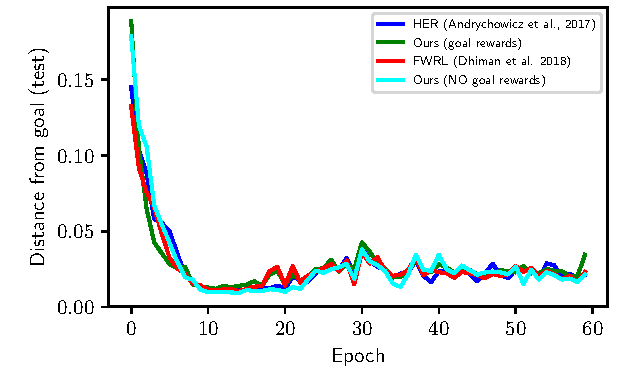
\includegraphics[width=\frac\columnwidth]{media/res/6efc1de-path_reward_low_thresh_chosen-FetchReachPR-v1-dqst/epoch-test/ag_g_dist.pdf}%
  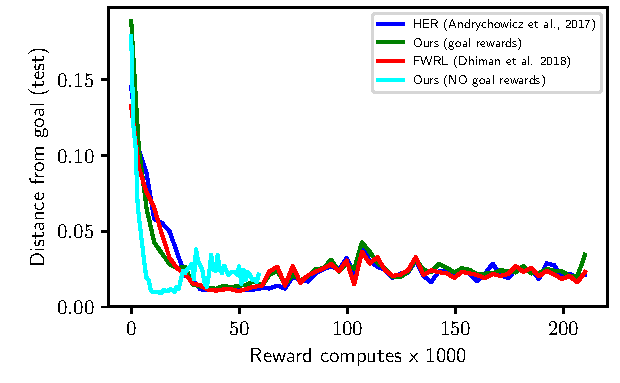
\includegraphics[width=\frac\columnwidth]{media/res/6efc1de-path_reward_low_thresh_chosen-FetchReachPR-v1-dqst/reward_computes-test/ag_g_dist.pdf}%
  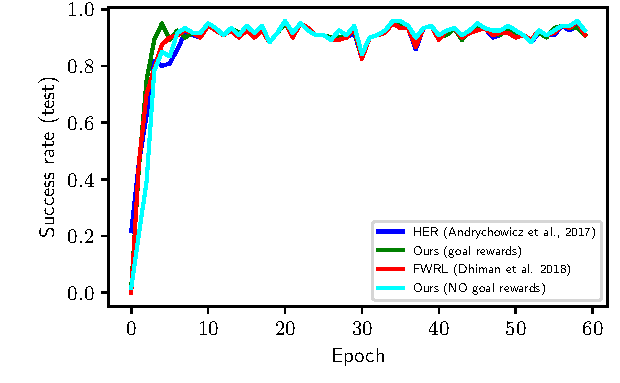
\includegraphics[width=\frac\columnwidth]{media/res/6efc1de-path_reward_low_thresh_chosen-FetchReachPR-v1-dqst/epoch-test/success_rate.pdf}%
  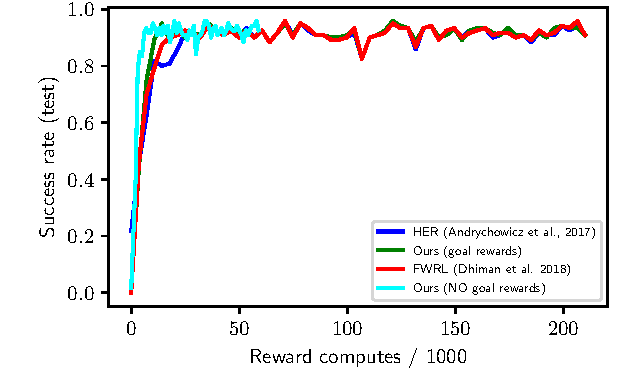
\includegraphics[width=\frac\columnwidth]{media/res/6efc1de-path_reward_low_thresh_chosen-FetchReachPR-v1-dqst/reward_computes-test/success_rate.pdf}\\
  \rotatebox{90}{\hspace{2em}\color{blue}{\tiny Fetch Push}}%
  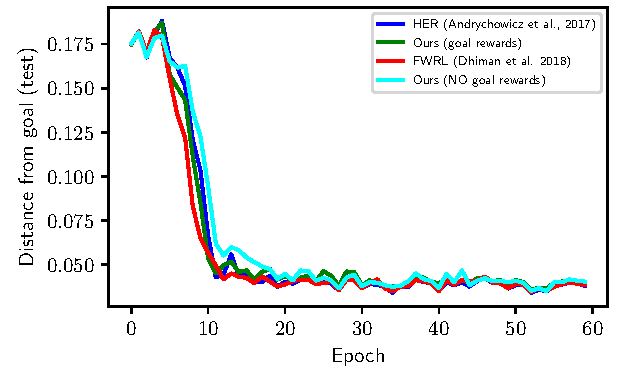
\includegraphics[width=\frac\columnwidth]{media/res/6efc1de-path_reward_low_thresh_chosen-FetchPushPR-v1-dqst/epoch-test/ag_g_dist.pdf}%
  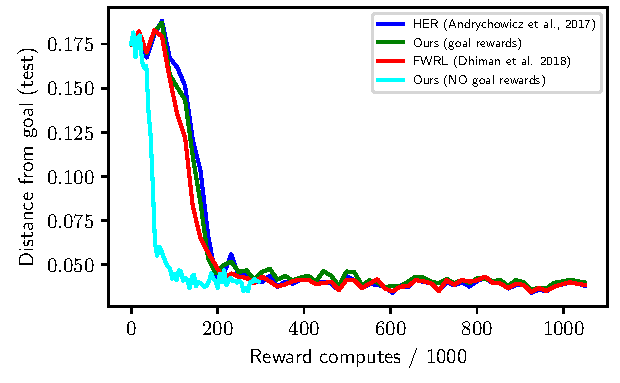
\includegraphics[width=\frac\columnwidth]{media/res/6efc1de-path_reward_low_thresh_chosen-FetchPushPR-v1-dqst/reward_computes-test/ag_g_dist.pdf}%
  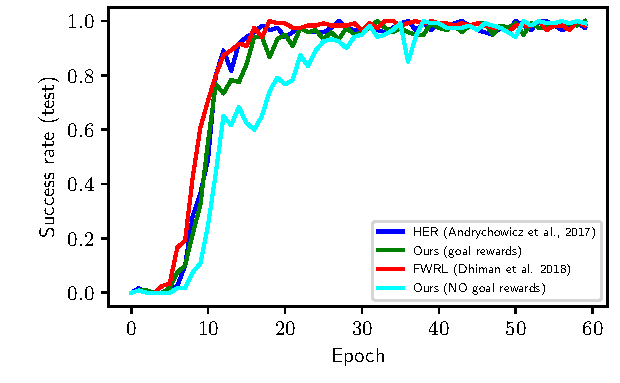
\includegraphics[width=\frac\columnwidth]{media/res/6efc1de-path_reward_low_thresh_chosen-FetchPushPR-v1-dqst/epoch-test/success_rate.pdf}%
  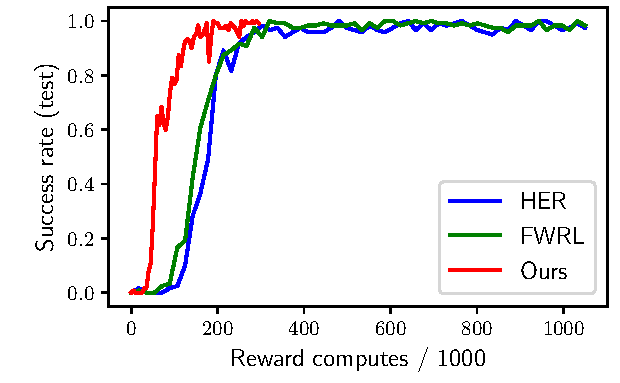
\includegraphics[width=\frac\columnwidth]{media/res/6efc1de-path_reward_low_thresh_chosen-FetchPushPR-v1-dqst/reward_computes-test/success_rate.pdf}\\
  \rotatebox{90}{\hspace{2em}\color{blue}{\tiny Fetch Slide}}%
  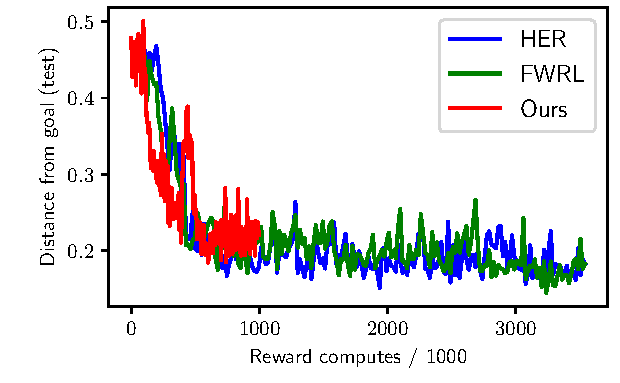
\includegraphics[width=\frac\columnwidth]{media/res/6efc1de-path_reward_low_thresh_chosen-FetchSlidePR-v1-dqst/reward_computes-test/ag_g_dist.pdf}%
  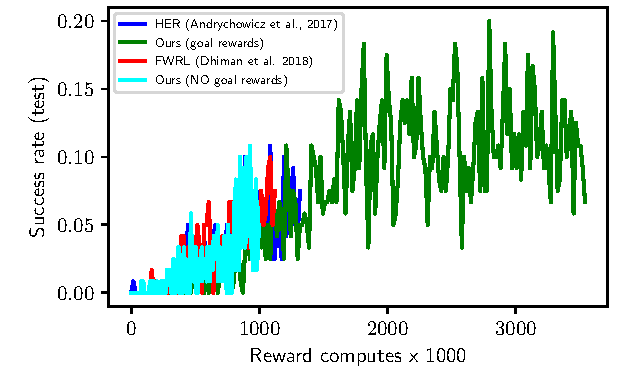
\includegraphics[width=\frac\columnwidth]{media/res/6efc1de-path_reward_low_thresh_chosen-FetchSlidePR-v1-dqst/reward_computes-test/success_rate.pdf}%
  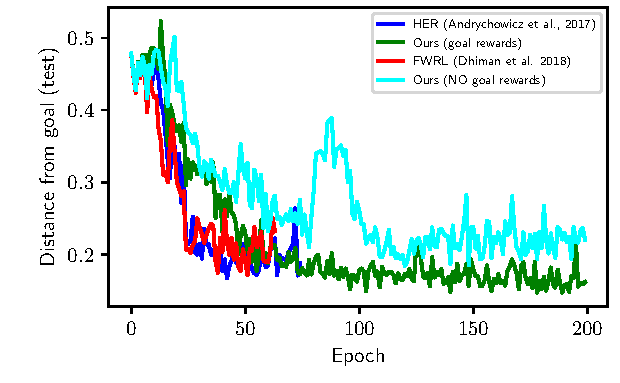
\includegraphics[width=\frac\columnwidth]{media/res/6efc1de-path_reward_low_thresh_chosen-FetchSlidePR-v1-dqst/epoch-test/ag_g_dist.pdf}%
  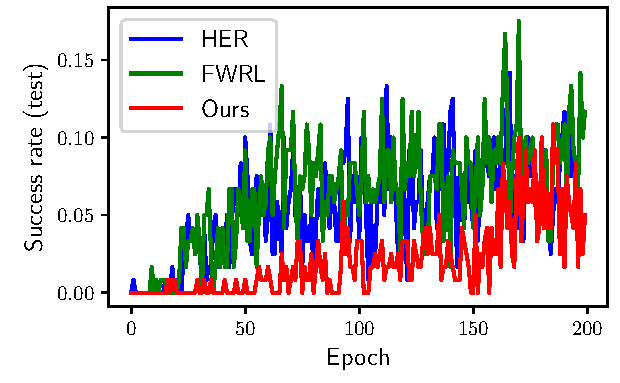
\includegraphics[width=\frac\columnwidth]{media/res/6efc1de-path_reward_low_thresh_chosen-FetchSlidePR-v1-dqst/epoch-test/success_rate.pdf}\\
  \rotatebox{90}{{\tiny \hspace{1em} \color{blue}{Fetch Pick And Place}}}%
  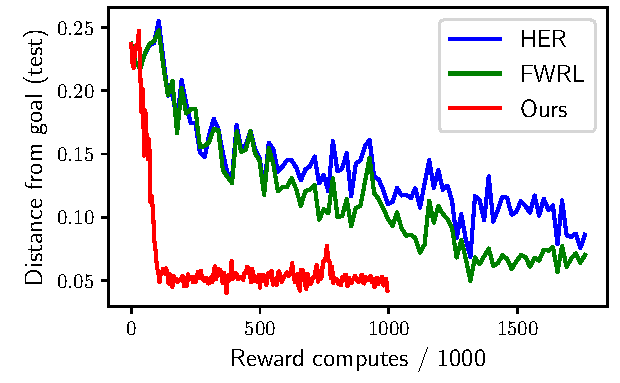
\includegraphics[width=\frac\columnwidth]{media/res/6efc1de-path_reward_low_thresh_chosen-FetchPickAndPlacePR-v1-dqst/reward_computes-test/ag_g_dist.pdf}%
  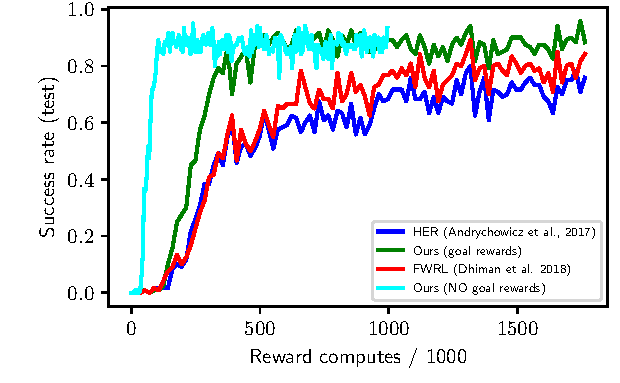
\includegraphics[width=\frac\columnwidth]{media/res/6efc1de-path_reward_low_thresh_chosen-FetchPickAndPlacePR-v1-dqst/reward_computes-test/success_rate.pdf}%
  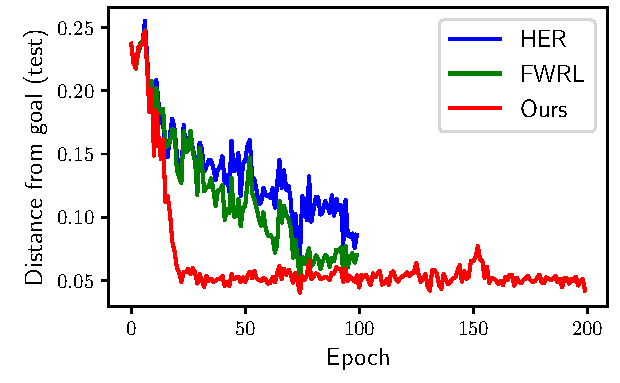
\includegraphics[width=\frac\columnwidth]{media/res/6efc1de-path_reward_low_thresh_chosen-FetchPickAndPlacePR-v1-dqst/epoch-test/ag_g_dist.pdf}%
  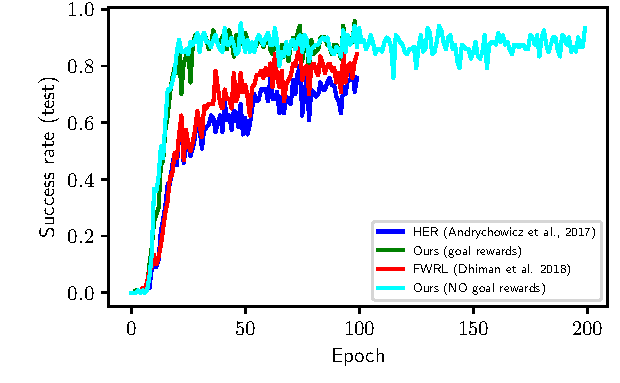
\includegraphics[width=\frac\columnwidth]{media/res/6efc1de-path_reward_low_thresh_chosen-FetchPickAndPlacePR-v1-dqst/epoch-test/success_rate.pdf}\\
  \label{fig:path-reward-fetch}%
  \caption{Effect of path reward on convergence in case of different algorithms
on Fetch tasks. Our method is able achieve similar performance even without the
goal rewards. Since our method without goal-rewards does not need reward
recomputation, we vastly outperform other methods in terms of reward sample
complexity.}%
\end{figure}

\subsubsection{Hand Tasks}


\begin{figure}
  \def\frac{0.24}
  \rotatebox{90}{{\tiny \hspace{1em} \color{blue}{Hand Reach}}}%
  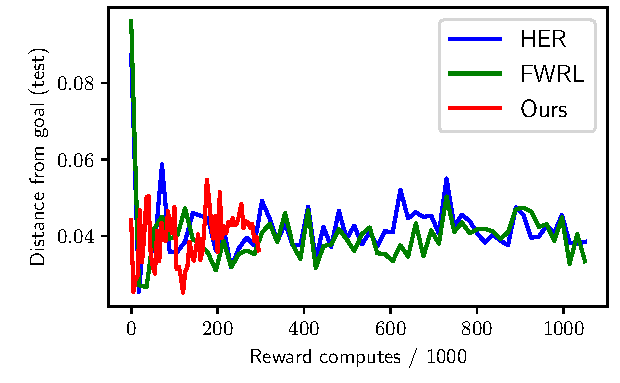
\includegraphics[width=\frac\columnwidth]{media/res/6efc1de-path_reward_low_thresh_chosen-HandReachPR-v0-dqst/reward_computes-test/ag_g_dist.pdf}%
  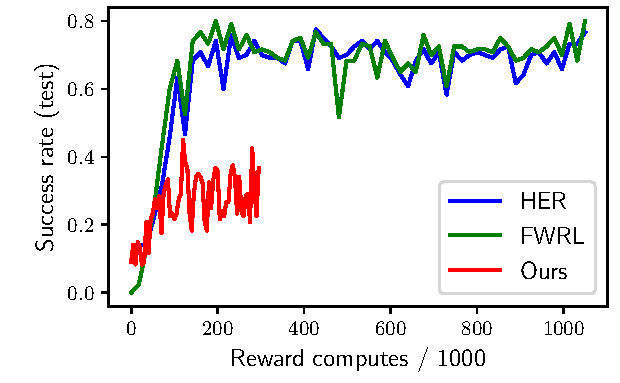
\includegraphics[width=\frac\columnwidth]{media/res/6efc1de-path_reward_low_thresh_chosen-HandReachPR-v0-dqst/reward_computes-test/success_rate.pdf}%
  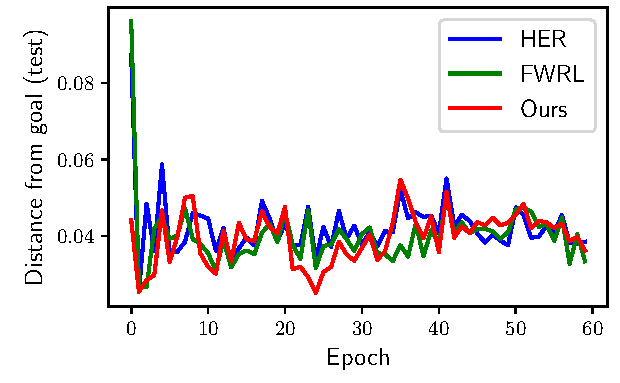
\includegraphics[width=\frac\columnwidth]{media/res/6efc1de-path_reward_low_thresh_chosen-HandReachPR-v0-dqst/epoch-test/ag_g_dist.pdf}%
  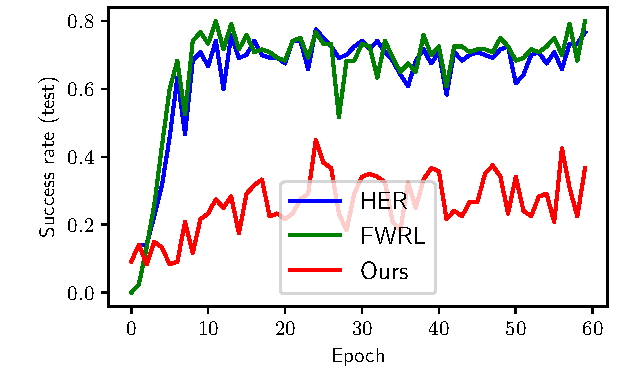
\includegraphics[width=\frac\columnwidth]{media/res/6efc1de-path_reward_low_thresh_chosen-HandReachPR-v0-dqst/epoch-test/success_rate.pdf}\\
  \rotatebox{90}{{\tiny \hspace{1em} \color{blue}{Hand Block Rotate}}}%
  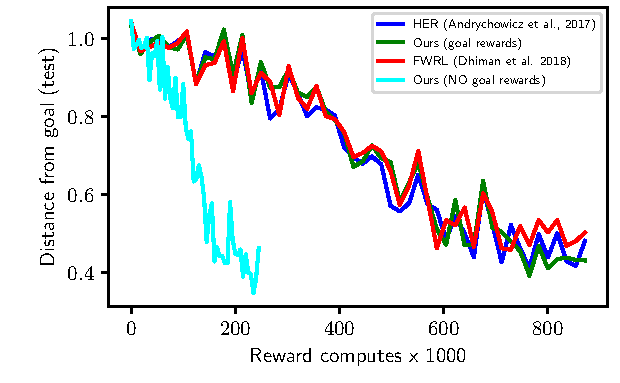
\includegraphics[width=\frac\columnwidth]{media/res/6efc1de-path_reward_low_thresh_chosen-HandManipulateBlockRotateXYZPR-v0-dqst/reward_computes-test/ag_g_dist.pdf}%
  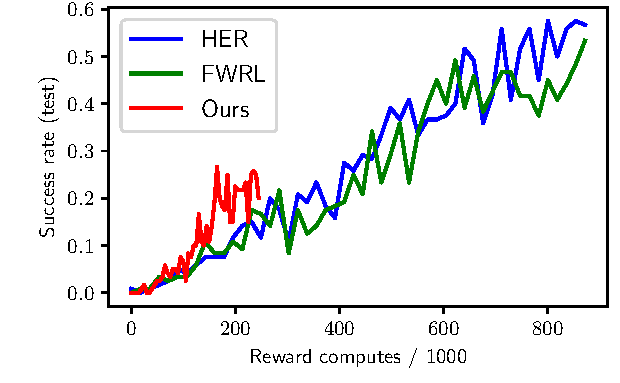
\includegraphics[width=\frac\columnwidth]{media/res/6efc1de-path_reward_low_thresh_chosen-HandManipulateBlockRotateXYZPR-v0-dqst/reward_computes-test/success_rate.pdf}%
  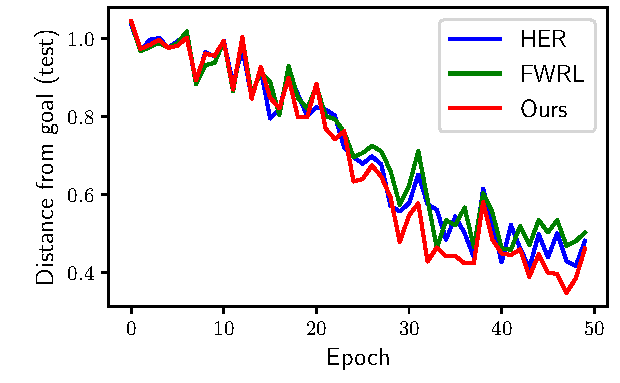
\includegraphics[width=\frac\columnwidth]{media/res/6efc1de-path_reward_low_thresh_chosen-HandManipulateBlockRotateXYZPR-v0-dqst/epoch-test/ag_g_dist.pdf}%
  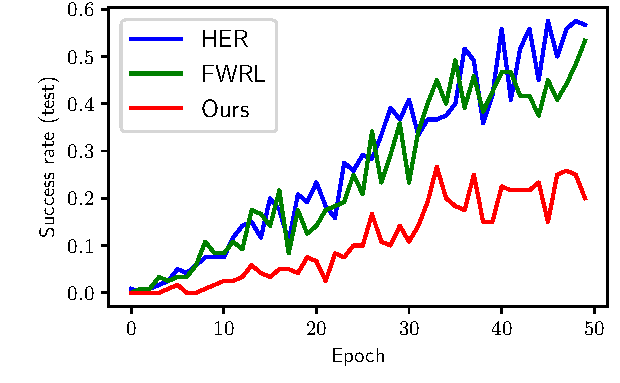
\includegraphics[width=\frac\columnwidth]{media/res/6efc1de-path_reward_low_thresh_chosen-HandManipulateBlockRotateXYZPR-v0-dqst/epoch-test/success_rate.pdf}\\
  \rotatebox{90}{{\tiny \hspace{1em} \color{blue}{Hand Egg}}}%
  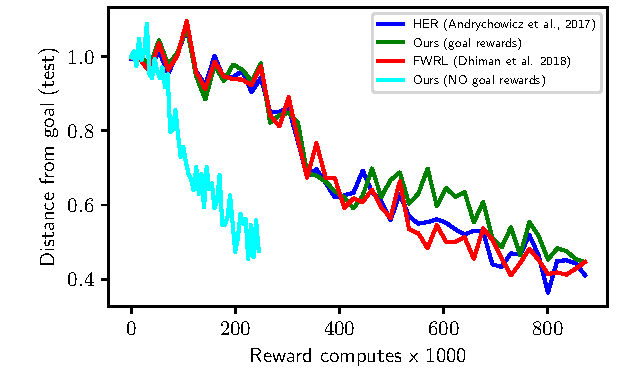
\includegraphics[width=\frac\columnwidth]{media/res/6efc1de-path_reward_low_thresh_chosen-HandManipulateEggFullPR-v0-dqst/reward_computes-test/ag_g_dist.pdf}%
  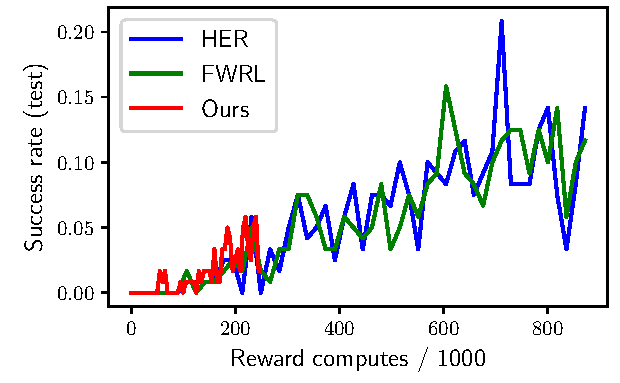
\includegraphics[width=\frac\columnwidth]{media/res/6efc1de-path_reward_low_thresh_chosen-HandManipulateEggFullPR-v0-dqst/reward_computes-test/success_rate.pdf}%
  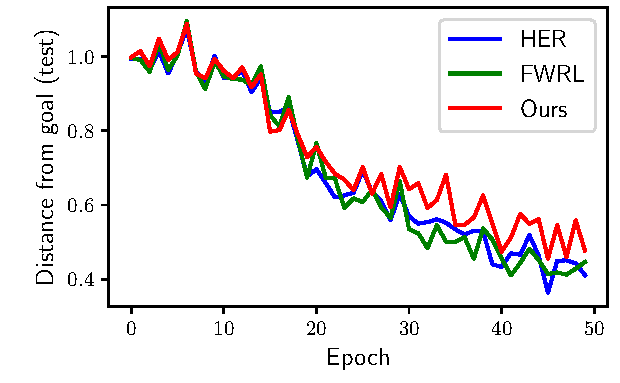
\includegraphics[width=\frac\columnwidth]{media/res/6efc1de-path_reward_low_thresh_chosen-HandManipulateEggFullPR-v0-dqst/epoch-test/ag_g_dist.pdf}%
  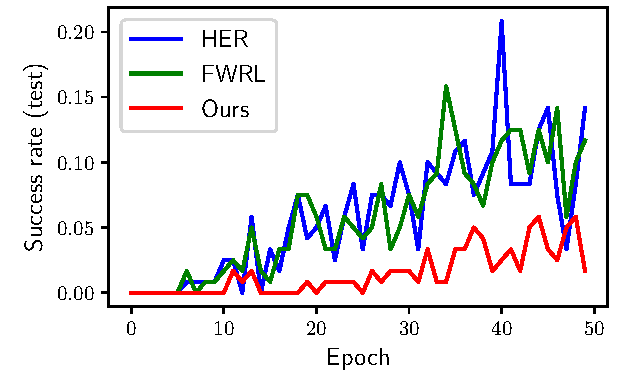
\includegraphics[width=\frac\columnwidth]{media/res/6efc1de-path_reward_low_thresh_chosen-HandManipulateEggFullPR-v0-dqst/epoch-test/success_rate.pdf}\\
  \rotatebox{90}{{\tiny \hspace{1em} \color{blue}{Hand Pen Rotate}}}%
  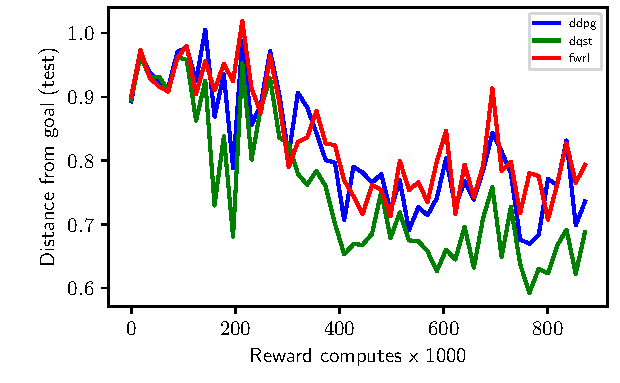
\includegraphics[width=\frac\columnwidth]{media/res/6efc1de-path_reward_low_thresh_chosen-HandManipulatePenRotate-v0-dqst/reward_computes-test/ag_g_dist.pdf}%
  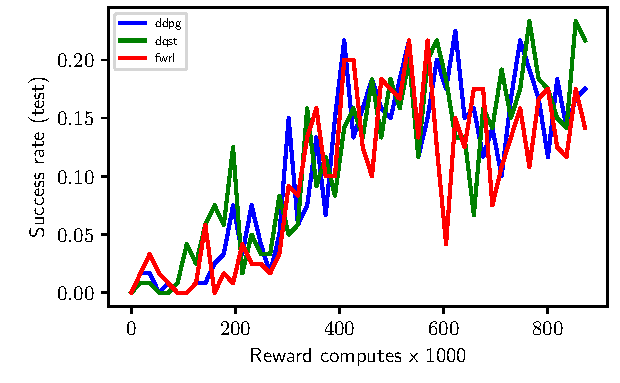
\includegraphics[width=\frac\columnwidth]{media/res/6efc1de-path_reward_low_thresh_chosen-HandManipulatePenRotate-v0-dqst/reward_computes-test/success_rate.pdf}%
  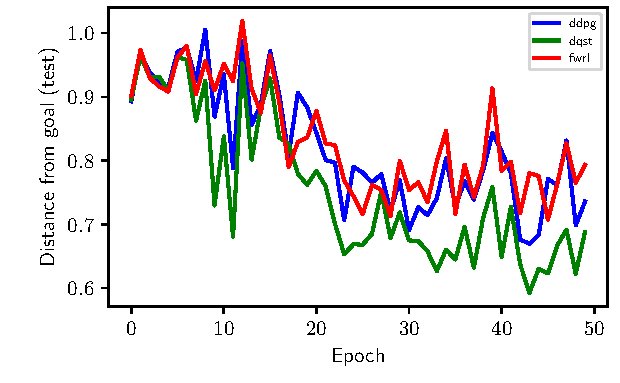
\includegraphics[width=\frac\columnwidth]{media/res/6efc1de-path_reward_low_thresh_chosen-HandManipulatePenRotate-v0-dqst/epoch-test/ag_g_dist.pdf}%
  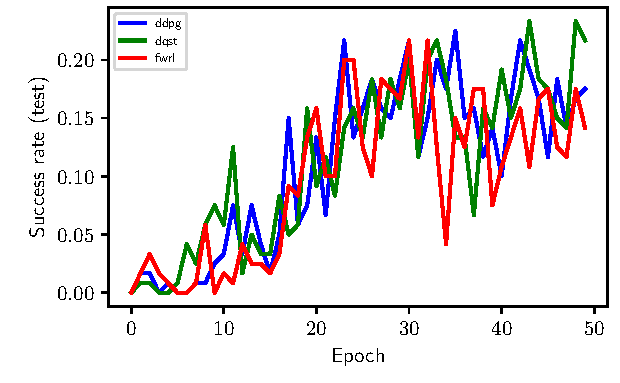
\includegraphics[width=\frac\columnwidth]{media/res/6efc1de-path_reward_low_thresh_chosen-HandManipulatePenRotate-v0-dqst/epoch-test/success_rate.pdf}\\
  \label{fig:path-reward-hand}%
  \caption{Effect of path reward on convergence in case of different algorithms
on Hand tasks. Our method is able achieve similar performance even without the
goal rewards. Since our method without goal-rewards does not need reward
recomputation, we vastly outperform other methods in terms of reward sample
complexity.}%
\end{figure}%
% 